% LATeX2e document

\documentclass[12pt]{article}
\pagestyle{empty}

\usepackage{tikz-cd}
\usepackage{amsmath,amssymb,amsfonts,bm}
\usepackage{stmaryrd}
\usepackage{bbold}
\usepackage{times}
\usepackage[all]{xy}
\usepackage{mathrsfs}
\usepackage{graphicx}
\usepackage{url}
\usepackage{pgfplots}
\usepackage{xcolor}
\usepackage{amsthm}
\usepackage[space]{grffile}

\graphicspath{ {C:/Users/Geoffrey/} }
\pgfplotsset{compat=1.12}
\textwidth 1.2\textwidth
\textheight 1.2\textheight
\topmargin 0in
\oddsidemargin 0in
\setlength{\topmargin}{0in}
\setlength{\headsep}{0in}
\setlength{\headheight}{0in}

%%%%%%%%%%%%%%%%%   definitions    %%%%%%%%%%%%%%%%%%%%%%%%%%%%%%%%%%%%

\newcommand{\FF}{\mathbb{F}}
\newcommand{\NN}{\mathbb{N}}
\newcommand{\ZZ}{\mathbb{Z}}
\newcommand{\QQ}{\mathbb{Q}}
\newcommand{\RR}{\mathbb{R}}
\newcommand{\CC}{\mathbb{C}}
\newcommand{\al}{\alpha}

\newcommand{\PaB}{\mathsf{PaB}}
\newcommand{\Calc}{\mathsf{Calc}}

\DeclareMathOperator{\Hom}{Hom}
\DeclareMathOperator{\Aut}{Aut}
\DeclareMathOperator{\Inn}{Inn}
\DeclareMathOperator{\Ker}{Ker}
\DeclareMathOperator{\Tor}{Tor}
\DeclareMathOperator{\Ext}{Ext}
\DeclareMathOperator{\Coker}{Coker}
\DeclareMathOperator{\Log}{log}

\newcommand{\onto}{\twoheadrightarrow}
\newcommand{\mono}{\rightarrowtail}
\newcommand{\into}{\hookrightarrow}
\newcommand{\tto}{\longrightarrow}
\newcommand{\iso}{\overset{\sim}{\tto}}
\newcommand{\impl}{\Rightarrow}
\newcommand{\conj}[1]{{}^#1}
\newcommand{\bigslant}[2]{\raisebox{.2em}{$#1$}\left/\raisebox{-.2em}{$#2$}\right.}

\newcommand{\bs}{\mspace{0mu}}
\newcommand{\ednote}[1]{\textcolor{red}{#1}}

\newcommand*{\octfont}{\fontfamily{cmvtt}\selectfont}

%\renewcommand{\labelenumi}{(\alph{enumi})}
\renewcommand{\labelenumi}{\textbf{(\alph{enumi})}}

\newtheorem{definition}{Definition}

\title{Identifying Tree Species via Photographs of Leaves}
\date{9 April 2017}
\author{Geoffrey E. Schneider}

\begin{document}

\maketitle
\section{Introduction} My primary objective in this project is to practice, learn and experiment with machine learning techniques, as well as to form a kind of portfolio of my personal knowledge and abilities in this area. The project objective is to identify tree species from photos of their leaves. Because my objective is not the same as the project objective, I will not always take the most direct approach to the problem, experimenting with techniques that might not be absolutely necessary. I will however, try to mimic good practices in developing machine learning algorithms. As such, I will start with the easiest approach to the easiest version of the problem as outlined below in Section \ref{sec:plans}, as a baseline from which to compare other algorithms.

This is a work in progress, as apparent by the empty sections below.

\section{Plans} \label{sec:plans}
\underline{Quick and dirty approach:}
\begin{enumerate}
 \item Gather a small amount of data (1 or 2 species, ~100 examples)
 \item Put data in a standard, usable form (minimal cleaning)
 \item Implement simple logistic regression
 \item Evaluate accuracy and ways to improve via learning curves and accuracy metric.
 \item Ceiling analysis (if appropriate).
\end{enumerate}

\noindent \underline{Additional models to try:}
\begin{itemize}
 \item Perceptron
 \item CNN
 \item SVM  
\end{itemize}

\noindent \underline{Data cleaning:}
\begin{itemize}
 \item PCA
 \item Autoencoder
 \item Background removal
 \item Feature choosing?
\end{itemize}

\noindent \underline{Additional data gathering:}
\begin{itemize}
 \item Manual data gathering
 \item Artificial data
 \item Other data repositories
\end{itemize}

\section{First Approach: Logistic Regression on Two Species} I begin by using the easiest possible approach to get results for comparison with later attempts. The first approach attempts to classify pictures of leaves from two species: \textit{Abies Concolor} and \textit{Abies Nordmanniana} using logistic regression. 

\subsection{Data} There were a total of 86 sample pictures of these leaves taken from the Leafsnap database \cite{leafsnap}. There were 51 for \textit{Abies Concolor} and 35 for \textit{Abies Nordmanniana} (See Figure \ref{fig:exphotos} for examples). They were color jpg photos.

\subsection{Preprocessing} The Octave script '{\octfont loadDataScript.m}' loads and preprocesses the images. Images were all approximately $600 \times 800$ pixels ($\pm 3$ pixels per dimension) when rotated such that the first dimension was shorter than the second. Because this would result in a very large feature vector, the size was reduced to $30 \times 40$ pixels for all images via the Octave command '{\octfont imresize}' from the '{\octfont image}' package. The $86$ resulting $30 \times 40 \times 3$ matrices were unrolled into a $86 \times 3600$ whose rows were randomly permutedm the data was normalized, and then divided into matrices of training data ({\octfont X}), cross-validation data ({\octfont X\_cv}) and test data ({\octfont X\_test}). These are labelled with corresponding vectors {\octfont y, y\_cv} and {\octfont y\_test}. The label {\octfont 0} corresponds to \textit{Abies Concolor} and {\octfont 1} to \textit{Abies Nordmanniana}.

\begin{figure} \label{fig:exphotos}
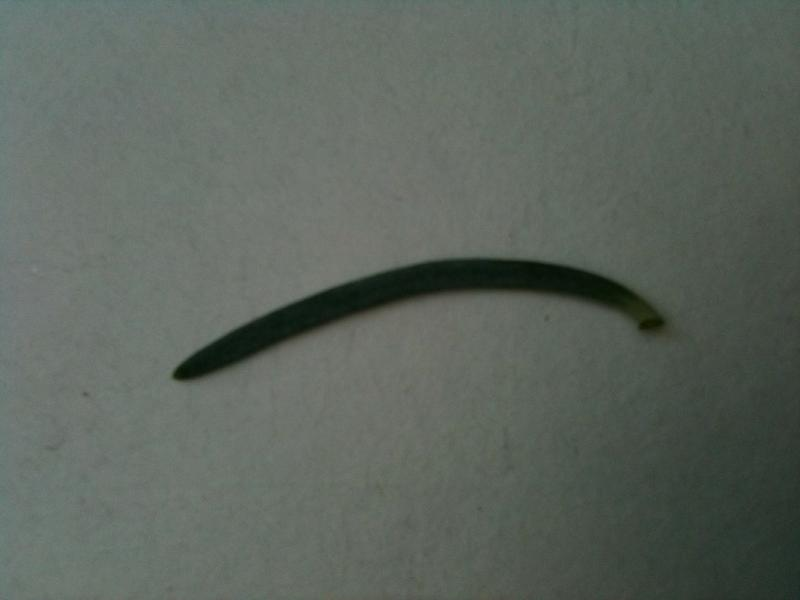
\includegraphics[scale=0.3]{C:/Users/Geoffrey/Documents/GitHub/MLproject/abies_concolor_ex.jpg} 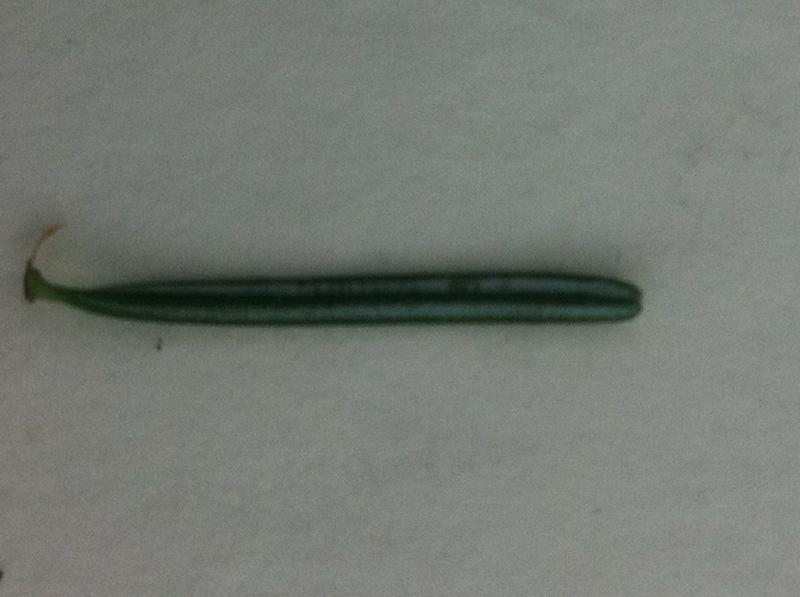
\includegraphics[scale=0.3]{C:/Users/Geoffrey/Documents/GitHub/MLproject/abies_nordmaniana_ex}
\caption{Example photos of Abies Concolor (left) and Abies Nordmanniana (right).}
\end{figure}

\subsection{Model} The model trained was a logistic regression model with regularization. The hypothesis for a particular example is given by:

\[
h_\theta(x) = \frac{1}{1+e^{x \cdot \theta}}
\]

Where $x$ is a feature vector and $\theta$ is a vector of the  model parameters.

The objective function is given by cross-entropy
\[
 J(\theta) = -\frac{1}{m}\sum_{i = 1}^m (y_i\Log(h_\theta(x_i))+(1-y_i)\Log(1-h_\theta(x_i)) + \frac{\lambda}{2m} \sum_{k=1}^n \theta_k^2
\]
where $y_i$ is the label and $x_i$ is the feature vector of the $i$th sample.

\subsection{Training} The model parameters were trained by minimizing cross-entropy using the Octave '{\octfont fminunc}' function, with theta initialized as the $0$ vector.

\subsection{Evaluation of results} The table below shows cost results for the model trained for various choices of the regularization parameter $\lambda$ (after training, cost was tested with $\lambda = 0$).

\begin{center}
\begin{tabular}{|l|c|c|c|c|}
 \hline
 $\lambda$ : & 0 & 0.1 & 0.3 & 1\\
 \hline
 training : & 1.3115e-004 & 0.0016223 & 0.0028836 & 0.0067081\\
 cross-validation: & 1.1418e-004 & 0.0023556 & 0.0015548 & 0.0019042 \\
 \hline
\end{tabular}
\end{center}

The pre-training cost was $0.69315$ on both the training set and the cross-validation set. If we predict \textit{Abies Concolor} when our hypothesis function gives a result $<0.5$, this gives a 100\% accuracy on the cross-validation set for all choices of $\lambda$. Figure \ref{fig:thetaZeroinitLogR} shows a visual representation of the model parameters (without the bias) when trained with $\lambda = 0$. 

The 100 \% accuracy clearly shows that the data is linearly separable, even with the large loss of information due to preprocessing. Because this simple model easily solves this problem, we must make the problem more difficult by including more species so that this can be a valid basis for comparison.

\begin{figure}
\begin{center} 
 
\includegraphics[scale=8]{C:/Users/Geoffrey/Documents/GitHub/MLproject/theta_im_zeroinit.png}
\end{center}
\caption{\label{fig:thetaZeroinitLogR} Visual representation of the trained parameters of the logistic regression model.}
\end{figure}

\subsection{Random Initialization} Using a random mean $0$, variance $1$ Gaussian initialization with $\lambda = 0$, we get an even lower cross-entropy of 1.4391e-006 on the cross-validation set. Figure \ref{fig:thetaRandinitLogR} shows that the model parameters train to radically different values in this case.

\begin{figure}
\begin{center}
 
\includegraphics[scale=8]{C:/Users/Geoffrey/Documents/GitHub/MLproject/theta_im_randinit.png}
\end{center} 
\caption{\label{fig:thetaRandinitLogR} Visual representation of the trained parameters of the logistic regression model with random initialization.}
\end{figure}

\subsection{More Species}


\begin{thebibliography}{99}
\bibitem{leafsnap} Neeraj Kumar, Peter N. Belhumeur, Arijit Biswas, David W. Jacobs, W. John Kress, Ida Lopez, Jo\~{a}o V. B. Soares, "Leafsnap: A Computer Vision System for Automatic Plant Species Identification," Proceedings of the 12th European Conference on Computer Vision (ECCV), October 2012.
\end{thebibliography}


\end{document}

